%!TEX root = Manuscrit.tex
\chapter{Généralisation}
\label{chap:generalisation}
%\citationChap{The purpose of computing is insight, not numbers.}{Richard Hamming}
\minitoc

\chapsummary{%

}

\newpage

\section{Cas des données limitées}

\subsection{Apprentissage par transfert}

VEDAI -> Potsdam/Christchurch

Potsdam <-> Vaihingen

Différences de radiométrie, de résolutions

\subsection{Génération de données synthétiques}

Comme nous l'avons vu dans le~\cref{chap:extension}, les jeux de données annotés en imagerie hyperspectrale sont rares et de petite taille. En effet, ceux-ci contiennent généralement peu d'exemples d'apprentissage en raison de la faible résolution des capteurs et de la complexité des annotations. Cependant, la précision des modèles d'apprentissage statistique augmente significativement avec le nombre d'échantillons. Une possibilité consiste donc à enrichir les jeux de données existants de façon artificielle, par un processus d'augmentation de données.

L'augmentation de données consiste à introduire des échantillons synthétiques afin d'enrichir un jeu d'apprentissage~\cite{dyk_art_2012}. Cette pratique est particulièrement courante pour l'entraînement des \gls{CNN} depuis l'article séminal de~\citet{krizhevsky_imagenet_2012} afin d'éviter le surapprentissage. Dans un contexte de classification de données hyperspectrales, la rareté des échantillons annotés rend l'augmentation de données d'autant plus attrayante. Cependant, la plupart des travaux de l'état de l'art appliquant des \gls{CNN} 2D ou 3D à la classification de telles images~\cite{chen_deep_2016,makantasis_deep_2015,slavkovikj_hyperspectral_2015,lee_contextual_2016} se sont limités à des jeux de données de taille restreinte, ne permettant pas d'exploiter au mieux les capacités d'apprentissage de représentation offertes par les réseaux profonds.

Ainsi, quelques études se sont penchées sur l'enrichissement artificiel des jeux de données hyperspectraux mis à la disposition de la communauté. \citet{windrim_hyperspectral_2016} ont proposé un modèle physique permettant de simuler les déformations d'un spectre s'il était soumis à des conditions d'illumination différentes de celle de l'acquisition originale, ce qui leur permet d'introduire une invariance à ces changements environnementaux. Toutefois, cela nécessite la conception et la mise en \oe{}uvre d'un modèle physique expert qui n'est pas générique, introduisant une phase d'estimation de l'illumination pouvant être imprécise dans des images de télédétection. Plus simplement, \citet{chen_deep_2016} augmentent le nombre d'échantillons disponibles en générant des combinaisons linéaires des spectres existants et en ajoutant du bruit gaussien. Enfin, \citet{acquarelli_convolutional_2017} proposent de propager les annotations d'un pixel à ses voisins par \emph{clustering} afin d'incorporer des pixels observés mais initialement non annotés dans le jeu d'apprentissage. Si cette approche permet en effet d'apprendre à partir de pixels supplémentaires, le nombre total d'échantillons est toutefois borné par la taille de l'image acquise.

Ainsi, nous introduisons la problématique suivante: comment enrichir les bases d'apprentissage lorsque aucun \emph{a priori} physique n'est disponible, en ajoutant autant de nouveaux échantillons que désiré? Une première piste de réponse se trouve dans les travaux de \citet{gemp_inverting_2017}. Ceux-ci implémentent des autoencodeurs variationnels qu'ils utilisent comme modèles génératifs pour le démélange de spectres, afin de déterminer les \emph{endmembers} d'une image.

Les modèles génératifs permettent en effet d'approximer les paramètres d'une distribution statistique latente à un ensemble d'observations pour en échantillonner de nouvelles. Nous proposons donc d'utilsier des modèles génératifs pour approximer la distribution latente des spectres au sein d'une image hyperspectrale afin de synthétiser de nouveaux échantillons susceptible d'appartenir à celle-ci. Il s'agit d'une approche ancrée uniquement dans les données, ne nécessitant aucun \emph{a priori} ou connaissance experte du capteur.

En particulier, nous proposons d'utiliser les \glspl{GAN}~\cite{goodfellow_generative_2014} afin d'approximer la distribution des spectres de l'image, puis d'en générer de nouveaux spectres dont la présence dans la distribution réelle est plausible. Afin de maximiser la quantité d'information exploitable, cette méthode se veut semi-supervisée afin de bénéficier aussi bien de la connaissance des spectres annotés que des spectres non-annotés. Nous validons l'intérêt d'utiliser ces spectres artificiels pour l'augmentation de données sur plusieurs jeux de données hyperspectraux publics, aériens comme satellitaires, sur différentes zones géographiques.

\section{Modèles génératifs adversaires}

\begin{figure}
		\resizebox{\textwidth}{!}{\begin{tikzpicture}
\usetikzlibrary{shapes.geometric}

\def \xgen {0}
\def \wblock {2}
\def \xdis {8}
\def \h {4}
\def \ydis {2}

\definecolor{blue}{RGB}{105, 150, 156}
\definecolor{red}{RGB}{170, 65, 57}
\definecolor{green}{RGB}{43, 130, 58}
\definecolor{orange}{RGB}{170, 111, 57}

% Générateur
\node [draw,trapezium, trapezium angle=75, shape border rotate=90,fill=blue!90!white, minimum width=3cm] (generator) at (1, 0) {\Large G};

% Discriminateur
\node [draw,trapezium, trapezium angle=75, shape border rotate=270,fill=green!50!white, minimum width=3cm] (discriminator) at (9, 2) {\Large D};
\node at (11.5, 2) (loss) {\small Réel/synthétique};
\draw[->,thick] (discriminator.east) -- (loss.west);

\node [draw,trapezium, trapezium angle=75, shape border rotate=270,fill=green!50!white, minimum width=3cm] (classifier) at (9, -2) {\Large C};
\node at (11.5, -2) (classes) {\small Classes};
\draw[->,thick,dashed] (classifier.east) -- (classes.west);
% Classifieur

% Bruit z
\node[rectangle, draw, rounded corners=6,fill=purple!50!white,minimum height=2.6cm] at (-1,1) (noise) {z};
\draw[->,thick,blue] (noise.east) to [bend right, out=0,in=-150] (generator.west);
% Condition
\node[rectangle, draw, rounded corners=6,fill=brown!50!white,minimum height=1cm] at (-1,-1) (condition) {c};
\draw[->,thick,blue] (condition.east) to [bend left, out=0,in=150] (generator.west);

% Spectres générés
\node[label={south:\footnotesize Spectres synthétiques}] at (\xgen+\wblock+2,0) (fake) {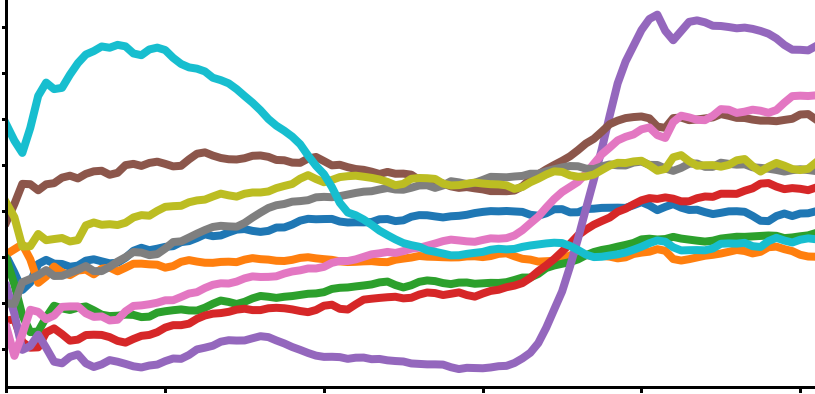
\includegraphics[width=2.5cm]{spectrum.png}};
\draw[->,thick,blue] (generator.east) -- (fake.west);
\draw[->,thick,blue] (fake.east) to [bend left=45,out=-25,in=-200] (discriminator.south west);
\draw [->, thick,blue,dashed] (fake.east) to [bend right=45,out=25,in=200] (classifier.north west) ;
% Jeu de données
\node [rectangle,draw,rounded corners=10, minimum width=3cm, minimum height=1cm,fill=gray!30!white] (unsupervised) at (4, 2) {\scriptsize Spectres non-étiquettés};
\node [rectangle,draw,rounded corners=10, minimum width=3cm, minimum height=1cm,fill=gray!30!white] (supervised) at (4, -2) {\scriptsize Spectres étiquettés};


\draw [->, thick,red] (unsupervised.east) -- node[above] {\footnotesize Spectres réels} (discriminator.west);
\draw [->, thick,red, dashed] (supervised.east) -- node[below] {\footnotesize Spectres réels} (classifier.west);
\draw [->, thick,red,dashed] (supervised.south) to [bend right=45, in=235] node[above] {\footnotesize Annotations} (classes.south west);
\draw [->, thick, blue,dashed] (condition.east) to [bend right=30, in=228] (classes.south);
\end{tikzpicture}
}
    \caption{La structure du \gls{GAN} utilisé pour la synthèse de spectres artificiels. Les flèches en \textcolor{BrickRed}{rouge} indiquent l'entraînement du classifieur et du discriminateur, tandis que les flèches en \textcolor{NavyBlue}{bleu} indiquent l'entraînement du générateur. Les flèches en pointillé indiquent les connexions qui ne sont utilisées que dans le cadre supervisé.}
    \label{fig:gan}
\end{figure}

Le principe des \glspl{GAN} a été introduit par~\citet{goodfellow_generative_2014} en 2014. L'idée est d'utiliser des réseaux de neurones profonds pour approximer la distribution statistique sous-jacente à un ensemble d'observations. Un générateur est ainsi entraîner pour approximer la transformation entre un espace latent de bruit gaussien vers la distribution empirique observée. Cependant, la distribution n'est observée que sur quelques échantillons et l'on souhaite utiliser le générateur pour créer de nouveaux échantillons probables.Pour ce faire, le générateur est entraîné pour approximer la distribution à l'aide d'une fonction objectif adversaire. Cette fonction est implicitement définie en introduisant un second réseau, appelé discriminateur ou critique. Le discriminateur apprend à estimer si un échantillon donné provient de l'ensemble des données réelles ou bien a été généré artificiellement. À chaque étape de l'optimisation, le discriminateur est entraîné sur quelques itérations afin de lui permettre d'estimer la frontière entre données réelles et données synthétiques. Le générateur est ensuite optimisé de telle sorte à ce qu'il \emph{piège} le discriminateur, c'est-à-dire que les échantillons synthétisés soient indistinguables des exemples réels du point de vue du critique.

Plusieurs variantes du cadre des \glspl{GAN} ont été proposées depuis leur introduction. Nous utilisons ici en particulier un générateur $G$ et un discriminateur $D$ utilisant le principe des Wasserstein \glspl{GAN}~\cite{arjovsky_wasserstein_2017} utilisant la régularisation de~\citet{gulrajani_improved_2017}, dont l'entraînement est prévu pour minimiser la distance de Wasserstein entre la distribution réelle et la distribution synthétique. Toutefois, ce mode de fonctionnement est non-supervisé, c'est-à-dire qu'il n'est possible que de générer de nouveaux échantillons sans contrôle sur leur classe. Il serait possible de créer un générateur pour chaque classe, mais cela serait coûteux en temps et en mémoire. Dans notre cas, nous souhaitons pouvoir \emph{conditionner} le générateur par rapport à la classe du spectre que nous souhaitons synthétiser. Nous utilisons ainsi un classifieur auxiliaire $C$~\cite{odena_conditional_2017} qui ajoute une contrainte supplémentaire lors de l'optimisation du générateur en s'assurant que les spectres générés sont bien classifiés dans la classe choisie.
L'architecture complète est détaillée dans la~\cref{fig:gan}. Si $G$ et $D$ peuvent être entraînés sans annotation, c'est-à-dire de façon non-supervisée, $C$ nécessite des échantillons annotés pour être entraîné. L'ensemble est donc semi-supervisé et peut exploiter simultanément les échantillons annotés disponibles et le reste de l'image.

\section{Experimental setup}
\label{sec:experimental_setup}

Nous entraînons ce \glspl{GAN} sur les jeux de données Pavia University, Pavia Center, Indian Pines et Botswana en utilisant les réflectances corrigées atmosphériquement lorsqu'elles sont disponibles. Comme nous essayons d'approximer des spectres individuels, nous utilisons pour $G$, $D$ et $C$ des réseaux simples entièrement connectés à 4 couches utilisant la fonction d'activation \emph{Leaky \gls{ReLU}}~\cite{maas_rectifier_2013}. La sortie de $G$ est suivie par une sigmoïde pour contraindre les valeurs de réflectance synthétisée entre $0$ et $1$. $D$ ne possède qu'une seule sortie et $C$ possède autant de sorties que le jeu de données a de classes.

L'optimisation des trois réseaux se fait en utilisant la politique de descente de gradient stochastique \emph{RMSProp}~\cite{rmsprop}. L'ensemble est entraîné durant 100 000 itérations avec une taille de \emph{batch} de 256, $C$ et $D$ étant entraînés 2 fois à chaque itération.

Par ailleurs, il apparaît nécessaire d'établir une performance de référence afin d'évaluer la pertinence des \glspl{GAN} pour la synthèse de spectres. Nous implémentons donc un modèle de mélange gaussien en utilisant la bibliothèque scikit-learn~\cite{pedregosa_scikit-learn_2011}. Nous reconstruisons un mélange pour chaque classe du jeu de données utilisant 10 composantes, que nous utilisons par la suite pour générer de nouveaux spectres.

\section{Spectra analysis}
\label{sec:analysis}

Dans un premier temps, nous cherchons à comparer selon plusieurs critères les distributions synthétiques et réelles. Pour ce faire, nous entraînons d'abord deux \glspl{GAN} sur Pavia University et Indian Pines.

\begin{figure}
\begin{subfigure}{0.5\textwidth}
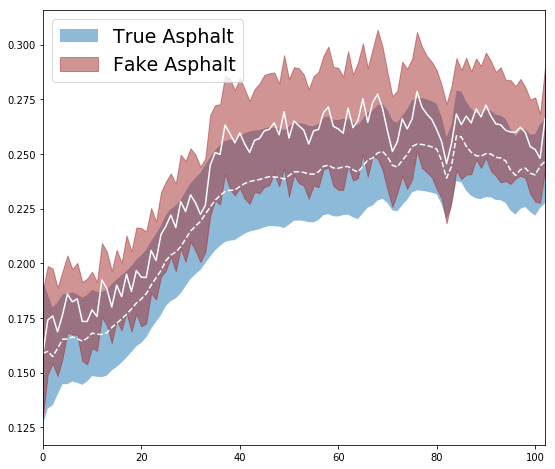
\includegraphics[width=\textwidth]{asphalt}
\end{subfigure}%
\begin{subfigure}{0.5\textwidth}
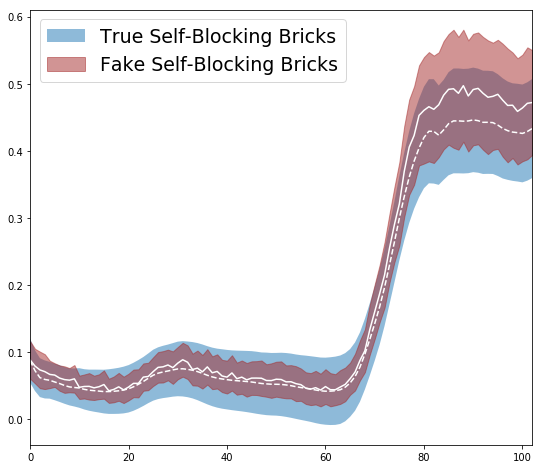
\includegraphics[width=\textwidth]{bricks}
\end{subfigure}
\caption{Spectre moyen et écart-type pour deux classes de matériaux du jeu de données Pavia Center. Les échantillons synthétiques moyens sont plus bruités et sont surappris sur certaines propriétés spectrales locales.}
\label{fig:mean_spectra}
\end{figure}

Visuellement, il est possible de constater dans la~\cref{fig:mean_spectra} que les spectres générés présentent des moments statistiques très similaires aux spectres réels. Les formes globales des spectres sont correctement approximés pour chaque classe. Toutefois, deux points négatifs sont identifiables. Tout d'abord, les spectres synthétiques moyens semblent plus bruités que leurs équivalents réels, ce qui signifie que le \gls{GAN} a surappris certaines particularités liées aux échantillons d'entraînement choisis. En outre, l'écart-type de la distribution synthétique est inférieur à celui de la distribution réelle, ce qui signifie que les faux spectres sont moins diversifiés que les vrais. Ces deux constatations indiquent que le générateur souffre partiellement d'une forme d'apprentissage appelée \emph{mode collapse}~\cite{salimans_improved_2016}.

\begin{figure}[t]
\begin{subfigure}{0.5\textwidth}
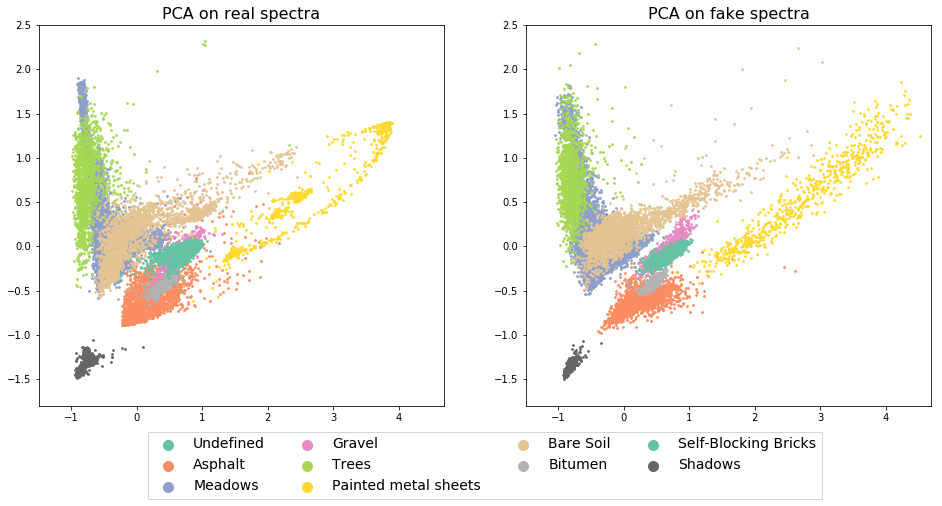
\includegraphics[width=\textwidth]{pca_paviau_acwgan}
\caption{Pavia University}
\end{subfigure}%
\begin{subfigure}{0.5\textwidth}
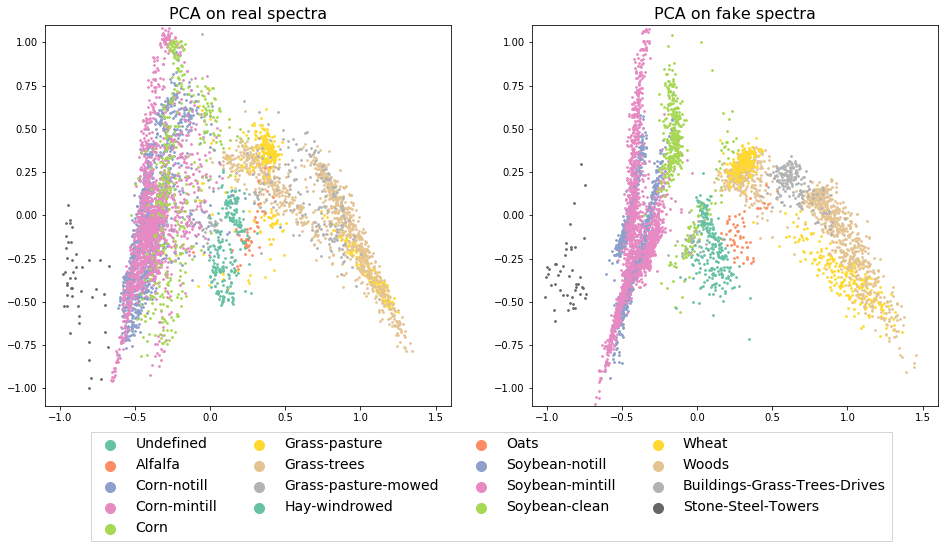
\includegraphics[width=\textwidth]{pca_indianpines_acwgan}
\caption{Indian Pines}
\end{subfigure}
\caption{\Gls{ACP} sur les spectres réels et synthétiques. Les spectres réels correspondent à l'ensemble des échantillons annotés de l'image. Les deux ensemble contiennent le même nombre d'éléments.}
\label{fig:pca}
\end{figure}

Pour mieux comprendre l'impact de ce surapprentissage, nous appliquons une \gls{ACP} afin de projeter les spectres réels et synthétiques dans un espace de représentation à deux dimensions (cf.~\cref{fig:pca}). Les groupes formés par les différentes classes sont correctement reproduits par les échantillons synthétiques. Cependant, la distribution synthétique présente également quelques déformations montrant que si le \gls{GAN} a bien réussi à modéliser la forme générale des différents types de spectres, il n'est cependant pas parvenu à reproduire l'ensemble de leurs spécificités.

\begin{table}[t]
	\begin{tabularx}{\textwidth}{c Y Y Y Y}
        Split & \multicolumn{2}{c}{Random (uniform)} & \multicolumn{2}{c}{Disjoint}\\
        \toprule
		\textbf{Train $\backslash$ Test} & Real & Fake & Real & Fake\\
        \midrule
        %\textbf{Train} & & & &\\
        Real & 89.5 & 98.3 & 87.2 & 98.8\\
        Fake & 87.8 & 99.2 & 79.4 & 99.9\\
        \bottomrule
	\end{tabularx}
    \caption{Exactitudes d'une \gls{SVM} linéaire appliquée sur les spectres réels et synthétiques du jeu de données Pavia University.}
    \label{table:svm_separation}
\end{table}

Nous pouvons essayer de construire une intuition sur la façon dont la distribution synthétique respecte les frontières entre classes de la distribution réelle en entraînant une \gls{SVM} linéaire sur les spectres réels et en l'appliquant pour séparer les spectres synthétiques. La \gls{SVM} va calculer les meilleurs hyperplans séparateurs pour la véritable distribution. Idéalement, ces hyperplans devraient séparer les spectres synthétiques exactement de la même façon. S'ils séparent nettement moins bien les spectres synthétiques, alors cela signifie que le générateur créé des échantillons irréalistes. S'ils séparent nettement mieux les échantillons, alors le générateur créé des exemples synthétiques trop similaires entre eux et regroupés autour des centroïdes corrsepondant aux classes réelles. Les résultats sont détaillés dans le~\cref{table:svm_separation}. Nous considérons deux approches\,: entraînement sur 3\% des spectres tirés au hasard uniformément ou sur 50\% de l'image, disjoint spatialement de la zone de validation. Dans le mode non-supervisé, nous utilisons également les échantillons non-annotés. Comme attendu, la \gls{SVM} sépare plus facilement les échantillons synthétiques que les spectres réels. Toutefois, entraîner la \gls{SVM} sur les spectres synthétiques uniquement permet tout de même de séparer les spectres réels dans une certaine mesure. Autrement dit, si les échantillons synthétiques sont moins diversifiés que les spectres réels, ils sont néanmoins représentatifs des différentes classes, et ce alors même que ces spectres sont générés \emph{ex nihilo} à partir de bruit aléatoire.

\begin{figure}[!t]
\begin{subfigure}{0.5\textwidth}
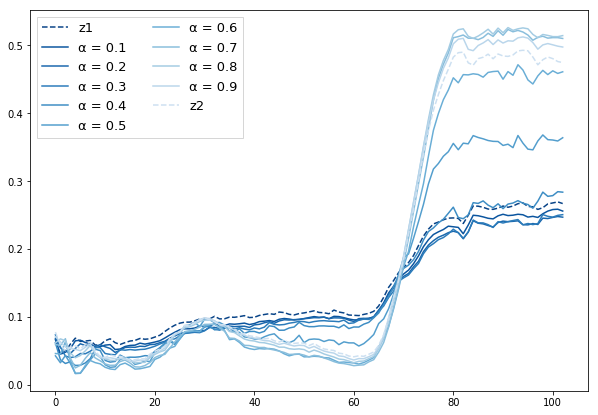
\includegraphics[width=0.95\textwidth]{interpolation_intraclass_acwgan}
\caption{Interpolation entre deux vecteurs latents de la classe ``sol nu''.}
\end{subfigure}%
\begin{subfigure}{0.5\textwidth}
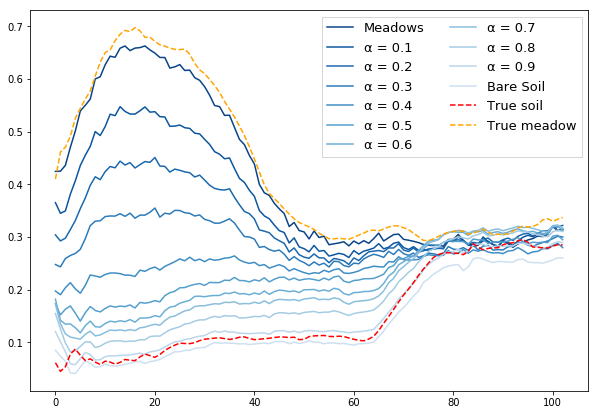
\includegraphics[width=0.95\textwidth]{interpolation_interclass_acwgan}
\caption{Interpolation à vecteur latent fixé entre les classes ``prairies'' et ``sol nu''.}
\end{subfigure}
\caption{Interpoler entre différents vecteurs ou conditionnements de l'espace latent permet d'explorer la variété des spectres de façon continue. Le \gls{GAN} est entraîné sur le jeu de données Pavia University. $\alpha$ contrôle l'interpolation.}
\label{fig:interpolation}
\end{figure}

Finalement, comme les \gls{GAN} permettent d'établir une projection entre un espace de représentation latent et le signal, il est possible d'explorer la variété des spectres en interpolant de façon continue entre deux points de l'espace latent. En particulier, il est également possible d'interpoler à vecteur de bruit fixe entre deux vecteurs de conditionnement. Ceci est illustré dans la~\cref{fig:interpolation}. Il existe une progression continue entre les échantillons générés, ce qui est particulièrement intéressant dans le cas de l'inteprolation entre classes. En effet, les spectres sont rarement purs et généralement constitués de mélanges, souvent non-linéaires, entre les réflectances de différents matériaux. Si les mélanges produits par le générateur sont réalistes, alors il effectue l'inverse de l'opération de démélange. Une approche d'apprentissage par dictionnaire, par inversion de modèle~\cite{gemp_inverting_2017} ou par plus proche voisin pourrait alors permettre, à partir d'un spectre réel soupçonné d'être un mélange, de revenir à ses \emph{endmembers} par une cartographie exhaustive de l'espace latent.

\begin{table*}[!t]
	\begin{tabularx}{\textwidth}{c c Y Y Y Y Y Y Y Y}
	\toprule
    \multicolumn{2}{c}{Dataset} & \multicolumn{2}{c}{PaviaU} & \multicolumn{2}{c}{PaviaC} & \multicolumn{2}{c}{Botswana} & \multicolumn{2}{c}{Indian Pines}\\
    Classifier & Augmentation & 3\% (r) & 50\% (s) & 3\% (r) & 50\% (s) & 3\% (r) & 50\% (s) & 3\% (r) & 50\% (s)\\
    \midrule
    \multirow{4}{*}{NN 1D} & $\emptyset$ & 92.72 & 86.22 & 98.93 & 96.26 & 86.90 & 84.87 & 79.44 & 74.00\\
    & GAN & 92.95 & 86.47 & 99.00 & 96.26 & 87.72 & 84.60 & 80.01 & 74.81\\
    & ss-GAN & 93.12 & 87.20 & 98.93 & 96.70 & 88.40 & 85.27 & 80.42 & 74.58\\
%     \midrule
%     \multirow{4}{*}{CNN 1D} & $\emptyset$ & - & - & - & - & - & - & - & -\\
%     & GAN & - & - & - & - & - & - & - & -\\
%     & ss-GAN & - & - & - & - & - & - & - & -\\
    \bottomrule
    \end{tabularx}
    \caption{Overall accuracies (OA) computed on several datasets with different data augmentation strategies. Sampling strategy is either a 50/50 spatial split of the image (s) or a uniform random sampling of 3\% of the labeled samples (r).}
    \label{table:da_results}
\end{table*}

\section{Data augmentation}
\label{sec:augmentation}

Les échantillons générés étant plausibles et représentatifs des spectres réels, nous suggérons de les utiliser pour enrichir les jeux de données annotés pré-existants. Nous testons cette idée sur plusieurs jeux de données : Indian Pines (aérien, rural), Pavia University (aérien, péri-urbain), Pavia Center (aérien, urbain) et Botswana (satellite, rural). Les résultats en mode supervisé et semi-supervisé sont détaillés dans le~\cref{table:da_results}. Augmenter le jeu de données à l'aide des faux spectres permet de légèrement augmenter les performances du classifieur.

Toutefois, augmenter drastiquement le nombre de faux spectres n'améliore pas plus la classification et finit même par la dégrader. En effet, dans ce cas les échantillons synthétiques deviennent prédominants dans la fonction de coût et dégradent les performances du classifieur, le ramenant vers le cas de la \gls{SVM} entraînée uniquement sur les faux spectres.

\section{Cas des données massives}

\subsection{Passage à l'échelle}

Supervisé mais large échelle

Jusqu'à présent, nous nous sommes intéressés à des jeux de données ne couvrant qu'une seule scène. En effet, les expériences des~\cref{chap:cartographie,chap:extension,chap:multimodal} ont été effectuées sur les villes de Vaihingen et Potsdam, pour une seule ville à la fois. Néanmoins, cela ne correspond pas à un cas applicatif réel. L'observation de la Terre passe par la répétition des acquisitions sur l'ensemble du globe. Par conséquent, il est nécessaire d'évaluer les capacités de généralisation des modèles mis en \oe{}uvre dans un cadre géographique varié.

\todo[inline]{inria aerial image labeling}

\todo[inline]{mini-france}

Nous collectons un jeu de données à large échelle sur la France métropolitaine. Nous utilisons la BD ORTHO de l'\gls{IGN} comme source d'images aériennes à une résolution de \SI{50}{\centi\meter/\px}. Les annotations du projet Copernicus \emph{Urban Atlas} 2012 sont utilisées, en complément des données \emph{Open Data} du cadastre français. Nous considérons les images de la BD ORTHO de 2012 à 2014 sous licence \emph{open data}. Nous filtrons hors du cadastre les bâtiments ajoutés à la base de données après le 1\ier janvier 2013.

Le jeu de données comprend finalement 16 agglomérations\,:




\todo[inline]{collab ESA}

%\bibliographystyle{plainnat}
%\bibliography{Chapitre5/Biblio}
\printbibliography
